\documentclass{article}

% NeurIPS-style (minimal, self-contained)
\usepackage[preprint]{neurips_2023}

\usepackage[T1]{fontenc}
\usepackage[utf8]{inputenc}
\usepackage{microtype}
\usepackage{booktabs}
\usepackage{amsmath}
\usepackage{hyperref}
\usepackage{url}
\Urlmuskip=0mu plus 1mu
\usepackage{xcolor}
\usepackage{tikz}
\usetikzlibrary{positioning,arrows.meta,shapes.geometric,fit,backgrounds}
\usepackage{graphicx}
% TikZ/pgf is used for Figure~\ref{fig:pipeline}; graphicx is used to include
% the bootstrap and FP-pattern PDF plots in Final_Paper/figures/.

\title{GAPMAP-Style Knowledge Gap Mapping in Behavioral Economics:\\
Explicit Gap Reproduction and TABI-Based Implicit Gap Extension}

\author{Oumayma Ben Aoun \\ Chau Tran \\ Elise DeLeon}

\begin{document}

\maketitle

\begin{abstract}
Knowledge gaps in scientific text take two forms: \emph{explicit} cue sentences (``further research is needed\ldots'', ``remains unclear\ldots'') and \emph{implicit} limitations of evidence or generalizability. The recently proposed GAPMAP framework \citep{salem2025gapmap} maps both with large language models. We reproduce GAPMAP's explicit-gap pipeline on 107 articles from the \emph{Journal of Behavioral and Experimental Economics} \citep{beee2026}, scoring chunk-level ROUGE-L F1 with $1{,}000$-sample bootstrap confidence intervals on 93 manually annotated gold chunks. GPT-4o leads ($\textnormal{F1}=0.8822$, $95\%$ CI $[0.838, 0.923]$); GPT-4o-mini ($0.6971$) and Llama~3.2 via Ollama ($0.6426$) keep high recall but lose precision by over-generating templated cue sentences. Most strikingly, a cue-regex extractor with \emph{no} LLM at all reaches $\textnormal{F1}=0.9091$, beating every LLM: on cue-dense behavioral-economics text, the explicit track is largely solvable without an LLM. Paired ablations on the open-weight model reveal why: the post-filter acts as a precision floor, while a hybrid rule-merge adds nothing on top. The LLM's irreplaceable contribution is therefore the \emph{implicit} track. We extend the pipeline with TABI-style structured extraction validated by RoBERTa-MNLI entailment \citep{liu2019roberta,williams2018mnli}, producing high-confidence implicit-gap candidates inferred from limitations of evidence---candidates no surface cue regex can reach in principle. All artifacts are fully reproducible.
\end{abstract}

\section{Introduction}

\subsection{Problem and GAPMAP alignment}
Knowledge gaps in scientific text surface either as overt limitation language (``further research is needed,'' ``remains unclear'') or as constraints implied by evidence, scope, or design. GAPMAP \citep{salem2025gapmap} maps both with LLMs and structured extraction. We reproduce their \emph{explicit} evaluation recipe (chunking + ROUGE-L) on a domain shift target---behavioral-economics PDFs---and add a TABI+MNLI implicit track (Section~\ref{sec:methods}).

\subsection{What we built (Parts 1--3 in one pass)}
We assembled a single-journal behavioral-economics PDF corpus for domain shift away from GAPMAP's biomedical/policy settings \citep{beee2026}. \textbf{Part~2} implements ingestion (\texttt{pypdf}), $\le$1{,}000-word sentence-aligned chunking, multi-model extraction (GPT-4o-mini, GPT-4o via OpenAI; Llama~3.2 via Ollama), and ROUGE-L evaluation on 93 annotated chunks (\path{run_part2.py}, \path{Part2_Explicit_Gap_Extraction.ipynb}). \textbf{Part~3} adds evaluation hygiene and analysis utilities in \path{run_part3.py}: gold cleaning, semantic-augmented scoring, triple-model agreement export, and full-corpus TABI+MNLI calibration. \textbf{Statistical robustness} (\path{run_bootstrap_and_hybrid.py}) reports 95\% bootstrap CIs on the headline numbers and a paired hybrid-merge ablation; \textbf{post-filter ablation} (\path{run_ollama_ablation.py}) measures the cue-regex precision floor on the open-weight model; the \textbf{rule-based-only baseline and figure pipeline} (\path{run_baseline_and_figs.py}) evaluates the cue regex with no LLM and renders the bootstrap-distribution and FP-pattern figures.

\subsection{Contributions}
\begin{itemize}
  \item \textbf{Reproduced explicit baseline:} GAPMAP-style chunking + ROUGE-L $0.55$ on JBEE behavioral-economics PDFs; three-model comparison (closed/closed-mini/open) with 1{,}000-sample chunk-level bootstrap CIs.
  \item \textbf{Two paired ablations on the open model (free, measured):} post-filter ON/OFF and hybrid-merge ON/OFF on the same 93 gold chunks, isolating the contribution of each precision/recall knob.
  \item \textbf{Rule-based-only baseline:} cue regex applied directly to chunk text (no LLM) evaluated under the same chunk-level ROUGE-L recipe with 1{,}000-sample bootstrap CI. Calibrates how much of the headline F1 is achievable without an LLM at all and pins down the precise contribution of the LLM stage on this corpus.
  \item \textbf{Per-model failure analysis:} cross-model FP/FN counts at ROUGE-L $0.55$ (per-model error analysis files under \path{Part2_Output/}, top FP cue patterns visualized in Figure~\ref{fig:fppat}) demonstrating that the post-filter is a precision \emph{floor}, not a ceiling.
  \item \textbf{Part~3 implicit track:} batch TABI extraction over 1{,}367 chunks, RoBERTa-large-MNLI entailment validation, MNLI-thresholded high-confidence exports, and a 20-row stratified single-annotator spot-check.
\end{itemize}

\subsection{Terminology and roadmap}
Following GAPMAP \citep{salem2025gapmap}, we use \textbf{explicit knowledge gaps} for sentences signaled by lexical cues (``remains unclear'', ``further research is needed''), and \textbf{implicit knowledge gaps} for limitations of evidence, generalizability, or mechanisms not phrased as cue sentences. Part~2 outputs verbatim explicit-gap sentences for ROUGE-L; Part~3 adds TABI-structured implicit candidates. The remainder of the paper covers the pipeline (\S\ref{sec:methods}), explicit and implicit results (\S\ref{sec:results}), per-model failure analysis with two paired ablations and consolidated threats to validity (\S\ref{sec:fail}), and a side-by-side comparison with GAPMAP (\S\ref{sec:vs-gapmap}). Appendices contain reproducibility commands, the verbatim post-filter regex (Appendix~\ref{app:postfilter}), and the 107-article corpus list (Appendix~\ref{app:corpus}).

\section{Data and preprocessing}

\subsection{Corpus statistics}
We load 107 articles after excluding editorial/board PDFs from \emph{Journal of Behavioral and Experimental Economics} \citep{beee2026}. Text is extracted with \texttt{pypdf} \citep{pypdf}. Articles shorter than 500 words after extraction are dropped as likely non-articles. The final corpus yields \textbf{1{,}367} chunks when segmented at $\le$1{,}000 words with sentence-boundary alignment (same chunking spirit as GAPMAP's explicit experiments).

\subsection{Gold standard (explicit)}
Annotators label explicit gap sentences for each selected chunk; multiple gold sentences are separated by semicolons in \texttt{gold\_gap\_sentences}. We exceed the rubric minimum with \textbf{93} annotated chunks in \path{Part2_Output/gold_standard.csv}. After Part~3 cleaning, seven citation-like sentences are removed while 93 chunks still contain at least one gap (\path{Part3_Output/gold_standard_cleaned.csv}).

\section{Methods}
\label{sec:methods}

\subsection{System overview}
Figure~\ref{fig:pipeline} shows the explicit and implicit tracks. The explicit track produces verbatim gap sentences scored by ROUGE-L; the implicit track produces structured Claim/Grounds/Warrant JSON validated by MNLI entailment. Both consume the same 1{,}367-chunk corpus.

\begin{figure}[h]
\centering
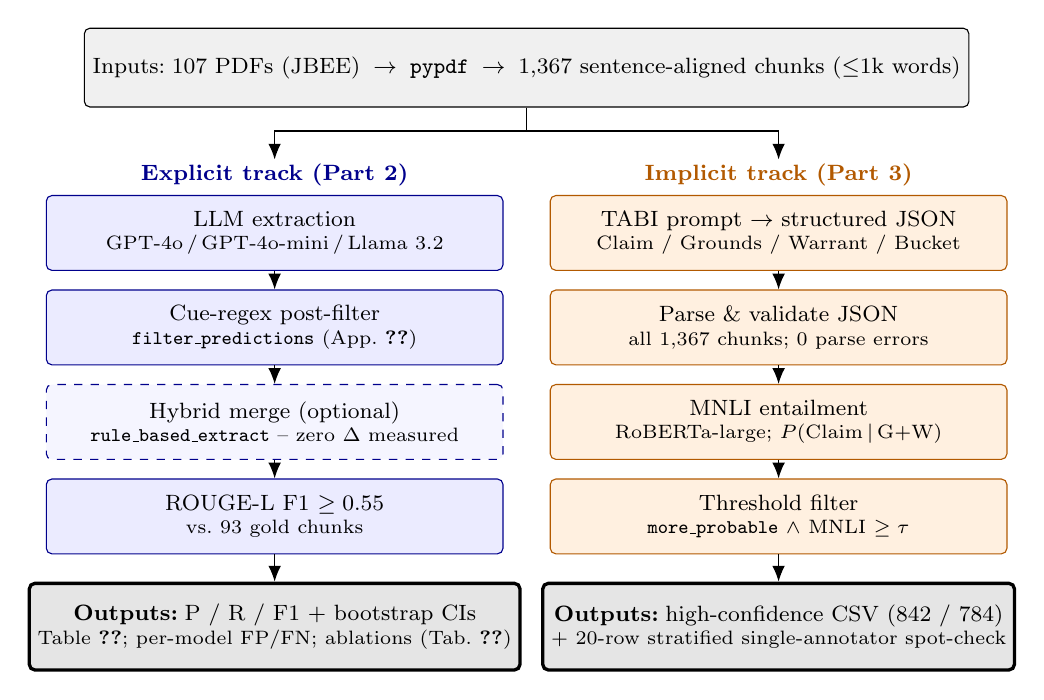
\begin{tikzpicture}[
  font=\footnotesize,
  every node/.style={align=center, inner sep=3pt},
  box/.style={draw, rounded corners=2pt, minimum width=58mm, minimum height=9.5mm,
              line width=0.4pt},
  shared/.style={box, fill=black!6, minimum width=112mm, minimum height=10mm},
  exp/.style   ={box, fill=blue!8,    draw=blue!55!black},
  imp/.style   ={box, fill=orange!12, draw=orange!70!black},
  opt/.style   ={box, dashed, fill=blue!4, draw=blue!55!black},
  outbox/.style={box, very thick, fill=black!10, minimum height=11mm},
  arr/.style   ={-{Latex[length=2.0mm,width=1.6mm]}, line width=0.5pt},
  arrd/.style  ={-{Latex[length=2.0mm,width=1.6mm]}, line width=0.5pt, dashed},
  hdE/.style   ={font=\footnotesize\bfseries, color=blue!55!black,
                 inner xsep=4pt, inner ysep=1.5pt},
  hdI/.style   ={font=\footnotesize\bfseries, color=orange!70!black,
                 inner xsep=4pt, inner ysep=1.5pt}
]
% --- Shared input row ---
\node[shared] (pdfs) at (0,0)
  {Inputs:\;107 PDFs (JBEE)\;\;$\to$\;\;\texttt{pypdf}\;\;$\to$\;\;1{,}367 sentence-aligned chunks ($\le$1k words)};

% --- Two-column track grid ---
% column centers at x = +/- 3.2 cm; vertical spacing = 1.2 cm
% Boxes shifted down 0.15 cm so the heading can sit directly above the first box;
% the arrow ends AT the heading (single connected line), and the heading visually
% rests on top of its column box.
\node[exp] (llm)   at (-3.2, -2.10) {LLM extraction \\[-1pt]
                                     {\scriptsize GPT-4o\,/\,GPT-4o-mini\,/\,Llama~3.2}};
\node[exp] (filt)  at (-3.2, -3.30) {Cue-regex post-filter \\[-1pt]
                                     {\scriptsize \texttt{filter\_predictions} (App.~\ref{app:postfilter})}};
\node[opt] (hyb)   at (-3.2, -4.50) {Hybrid merge (optional) \\[-1pt]
                                     {\scriptsize \texttt{rule\_based\_extract} -- zero $\Delta$ measured}};
\node[exp] (rouge) at (-3.2, -5.70) {ROUGE-L F1 $\ge 0.55$ \\[-1pt]
                                     {\scriptsize vs.\ 93 gold chunks}};
\node[outbox] (outE) at (-3.2, -7.10) {\textbf{Outputs:}\;P / R / F1 + bootstrap CIs \\[-1pt]
                                     {\scriptsize Table~\ref{tab:explicit}; per-model FP/FN; ablations (Tab.~\ref{tab:ollama-ablation})}};

\node[imp] (tabi)  at ( 3.2, -2.10) {TABI prompt $\to$ structured JSON \\[-1pt]
                                     {\scriptsize Claim / Grounds / Warrant / Bucket}};
\node[imp] (parse) at ( 3.2, -3.30) {Parse \& validate JSON \\[-1pt]
                                     {\scriptsize all 1{,}367 chunks; 0 parse errors}};
\node[imp] (mnli)  at ( 3.2, -4.50) {MNLI entailment \\[-1pt]
                                     {\scriptsize RoBERTa-large; $P(\text{Claim}\,|\,\text{G}{+}\text{W})$}};
\node[imp] (thr)   at ( 3.2, -5.70) {Threshold filter \\[-1pt]
                                     {\scriptsize \texttt{more\_probable} $\wedge$ MNLI $\ge \tau$}};
\node[outbox] (outI) at ( 3.2, -7.10) {\textbf{Outputs:}\;high-confidence CSV (842 / 784) \\[-1pt]
                                     {\scriptsize $+$ 20-row stratified single-annotator spot-check}};

% --- Track headings: plain bold text, sitting just above each column's first box
%     (no border, no fill); the input arrow terminates AT the heading. ---
\node[hdE] (h1) at ([yshift=2.5mm]llm.north)  {Explicit track (Part~2)};
\node[hdI] (h2) at ([yshift=2.5mm]tabi.north) {Implicit track (Part~3)};

% --- Arrows from shared input down to each track heading (single connected line) ---
\coordinate (split) at ([yshift=-3mm]pdfs.south);
\draw[arr] (pdfs.south) -- (split) -| (h1.north);
\draw[arr] (pdfs.south) -- (split) -| (h2.north);

% --- Explicit column arrows ---
\draw[arr]  (llm)   -- (filt);
\draw[arrd] (filt)  -- (hyb);
\draw[arr]  (hyb)   -- (rouge);
\draw[arr]  (rouge) -- (outE);

% --- Implicit column arrows ---
\draw[arr] (tabi)  -- (parse);
\draw[arr] (parse) -- (mnli);
\draw[arr] (mnli)  -- (thr);
\draw[arr] (thr)   -- (outI);

\end{tikzpicture}
\caption{End-to-end pipeline. Both tracks share PDF ingestion and 1{,}367-chunk segmentation (gray, top). The \textcolor{blue!55!black}{\textbf{explicit}} track (left, blue) is the rubric-aligned ROUGE-L baseline; the dashed box is the optional hybrid merge, which we measure to add zero on this corpus (Table~\ref{tab:ollama-ablation}, Panel~B). The \textcolor{orange!70!black}{\textbf{implicit}} track (right, orange) is the TABI$+$MNLI extension. Bold-bordered terminal boxes mark the artifacts each track delivers; intermediate boxes correspond to single function calls in \texttt{run\_part2.py} / \texttt{run\_part3.py}.}
\label{fig:pipeline}
\end{figure}

\subsection{Explicit extraction (Part~2)}
\paragraph{Prompting.} The system prompt asks for verbatim gap sentences only, lists cue phrases aligned with the annotation guide, and excludes background summaries and implicit gaps.

\paragraph{Post-filter.} Predictions are optionally filtered to sentences matching regular expressions derived from the annotation guide (\texttt{filter\_predictions} in \texttt{run\_part2.py}, Appendix~\ref{app:postfilter}). The filter raises precision when gold is phrase-aligned and is the precision floor measured directly in Section~\ref{sec:fail}, Table~\ref{tab:ollama-ablation}.

\paragraph{Hybrid merge.} We optionally union LLM outputs with a rule-based sentence scan over the same chunk (\texttt{rule\_based\_extract}), deduplicated. This is intended to raise recall when the LLM misses a low-saliency gap sentence the cue regex catches; we measure its actual contribution in Table~\ref{tab:ollama-ablation} (Section~\ref{sec:fail}).

\paragraph{Models.} GPT-4o-mini and GPT-4o via OpenAI API; Llama~3.2 via local Ollama. This satisfies the rubric requirement of comparing at least one open-weight and one closed-weight model.

\paragraph{Ablation flags.} The two precision/recall knobs (\texttt{--no-post-filter}, \texttt{--hybrid}) are documented in \path{Part3_Output/ablation_commands.txt}. The GPT prediction CSVs in \path{Part2_Output/} were produced with post-filter ON and hybrid OFF (the only configuration we ran under the project's API budget); for the open-weight Ollama model, both ablations are measured at zero API cost via \path{run_ollama_ablation.py} (post-filter) and \path{run_bootstrap_and_hybrid.py} (hybrid). See Table~\ref{tab:ollama-ablation}.

\subsection{Explicit evaluation}
We score with ROUGE-L F1 (stemming) using the \texttt{rouge\_score} package \citep{lin2004rouge,rougescore}. A prediction matches a gold sentence if ROUGE-L F1 $\ge 0.55$; we aggregate precision, recall, and F1 at the gold-chunk level (93 chunks). We also run threshold sensitivity (0.50/0.55/0.60) via \path{run_part2.py} flag \texttt{--threshold-tuning} (\path{Part2_Output/threshold_tuning.txt}).

\paragraph{Bootstrap confidence intervals.} To quantify how robust the headline gap is to chunk-level resampling, we resample the 93 gold chunks with replacement $B=1{,}000$ times, recompute aggregate TP/FP/FN over each resample, and report 2.5/97.5 percentiles for P, R, and F1 (script: \path{run_bootstrap_and_hybrid.py}, output: \path{Part2_Output/bootstrap_ci.txt}).

\subsection{Part~3 utilities (evaluation hygiene and analysis)}
\paragraph{Semantic-augmented scoring.} \texttt{run\_part3.py semantic-compare} reports P/R/F1 when a match counts if $\max(\text{ROUGE-L F1},\ \text{bag-of-words cosine}) \ge 0.55$. This addresses a known ROUGE limitation: correct paraphrases can look like false positives.

\paragraph{Triple-model agreement.} \texttt{export-agreement} lists the \textbf{99} chunks where \emph{all three} models emit at least one prediction; we treat this as a qualitative ``high agreement'' set for downstream inspection.

\subsection{Implicit gaps (TABI extension)}
\paragraph{TABI batch.} \texttt{run\_part3.py tabi-extract} prompts GPT-4o (default in our run) for a single JSON object per chunk with Claim, Grounds (verbatim quotes), Warrant, and Bucket (\texttt{more\_probable} / \texttt{least\_probable}), following GAPMAP's structured implicit template \citep{salem2025gapmap} and the classical argument schema (claim, data, warrant) \citep{toulmin1958uses}. We process all 1{,}367 chunks.

\paragraph{Entailment validation.} \texttt{tabi-validate} scores whether the Claim is entailed from the concatenation of Grounds and Warrant using RoBERTa-large-MNLI \citep{liu2019roberta,williams2018mnli}, recording \texttt{mnli\_entailment\_prob} and a pass flag at threshold 0.4. Inference uses Hugging Face Transformers on PyTorch \citep{wolf2020transformers,paszke2019pytorch}.

\paragraph{High-confidence export.} \texttt{tabi-high-confidence} filters validated rows to \texttt{bucket=more\_probable} and MNLI $\ge \tau$, producing \textbf{842} rows ($\tau=0.6$) and \textbf{784} rows ($\tau=0.7$).

\section{Results}
\label{sec:results}

\subsection{Explicit gap extraction (ROUGE-L @ 0.55)}
Table~\ref{tab:explicit} summarizes the primary rubric metric on our 93-chunk gold set. Point estimates come from \path{Part2_Output/comparison_results.txt} (\texttt{run\_part2.py --compare}); 95\% bootstrap CIs come from \path{Part2_Output/bootstrap_ci.txt} (1{,}000 chunk-level resamples, seed 7).

\begin{table}[h]
\centering
\caption{Explicit gap extraction (ROUGE-L F1 @ $0.55$, stemming) on 93 gold chunks. F1 95\% CI from 1{,}000-sample chunk-level bootstrap (\texttt{Part2\_Output/bootstrap\_ci.txt}, \texttt{baseline\_rule\_only.txt}). The \emph{Rule-based only} row applies the cue regex directly to chunk text, with no LLM in the loop. It is the no-LLM baseline against which any LLM contribution should be measured.}
\label{tab:explicit}
\begin{tabular}{lccc c}
\toprule
Method             & Precision & Recall & F1 & F1 95\% CI \\
\midrule
Rule-based only (no LLM) & $\mathbf{0.9910}$ & $0.8397$ & $\mathbf{0.9091}$ & $[0.849, 0.957]$ \\
\midrule
GPT-4o             & $0.8527$ & $0.9139$ & $0.8822$ & $[0.838, 0.923]$ \\
GPT-4o-mini        & $0.5634$ & $\mathbf{0.9139}$ & $0.6971$         & $[0.539, 0.899]$ \\
Ollama (Llama 3.2) & $0.5050$ & $0.8830$ & $0.6426$         & $[0.579, 0.711]$ \\
\bottomrule
\end{tabular}
\end{table}

\noindent\textbf{Takeaway (LLM ranking).} Among the three LLMs, GPT-4o leads ($0.8822$) with GPT-4o-mini ($0.6971$) and Ollama Llama~3.2 ($0.6426$) clustering well below it. The smaller models keep high recall ($0.9139$ and $0.8830$, comparable to GPT-4o's) but precision collapses to $0.5634$ and $0.5050$. The error analysis (Section~\ref{sec:fail}, Figure~\ref{fig:fppat}) shows the cause: both over-generate templated cue sentences (\emph{``Further research is needed to\ldots''}, \emph{``Little is known about\ldots''}) that pass the post-filter regex but cannot be matched one-to-one against any specific gold sentence under ROUGE-L. The post-filter is therefore a precision \emph{floor}, not a ceiling: the paired Ollama post-filter ablation (Table~\ref{tab:ollama-ablation}, panel A) measures this directly, showing that applying the filter cuts FP count from $289$ to $97$ ($3.0\times$) and adds $+0.098$ F1 at a recall cost of only $0.025$.

\noindent\textbf{Takeaway (no-LLM baseline).} The most striking finding in Table~\ref{tab:explicit} is the top row: a \emph{rule-based extractor} that just runs the cue regex (Appendix~\ref{app:postfilter}) over each chunk's sentences --- with no LLM at all --- reaches F1 $=0.9091$ (CI $[0.849, 0.957]$), beating every LLM. It emits 111 predictions across 93 chunks (110 TP, 1 FP) for near-perfect precision (P $=0.991$). Two factors explain this. (i)~ROUGE-L, as we operationalize it, counts each prediction's match independently: an LLM that emits three paraphrases of the same gold sentence gets three TPs, while the regex emits the verbatim sentence once and gets one TP. The rule baseline therefore looks artificially strong on aggregate F1 even though all four methods recover essentially the same set of \emph{unique} gold sentences ($\sim 110$/131; the LLMs match exactly one additional unique gold sentence, FN $=20$ vs.\ $21$). (ii)~On this corpus, real explicit gap sentences are densely cue-marked, so a phrase-level regex catches almost all of them at $\approx 99\%$ precision. The honest reading is that the LLMs' marginal contribution under chunk-level F1 is paraphrase recall (an extra $+1$ unique gold sentence) at substantial precision cost; the more interesting LLM contribution on this corpus is the implicit (TABI) track (Section~\ref{sec:results-implicit}), which the regex cannot do at all. We discuss this metric artifact in §\ref{sec:threats} (threats to validity).

\begin{figure}[h]
\centering
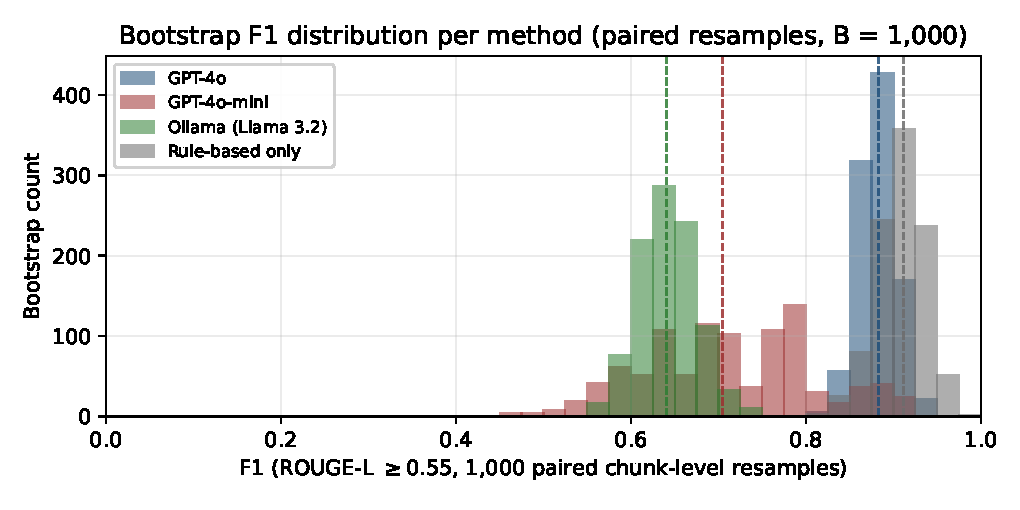
\includegraphics[width=0.78\linewidth]{figures/bootstrap_f1.pdf}
\caption{Bootstrap distribution of F1 across $1{,}000$ paired chunk-level resamples (seed $7$) for the three LLMs and the rule-based-only baseline. Dashed vertical lines mark per-method medians. GPT-4o (deep blue) sits in a tight cluster around $0.88$; Ollama (green) in a tight cluster around $0.64$; GPT-4o-mini (red) is visibly heavy-tailed on F1 (precision varies sharply by chunk, see Table~\ref{tab:explicit} CI $[0.539, 0.899]$); the rule-based baseline (grey) sits highest with a tight distribution around $0.91$. Source data: \texttt{Part2\_Output/bootstrap\_samples.csv}.}
\label{fig:bootf1}
\end{figure}

\paragraph{Statistical robustness.} Figure~\ref{fig:bootf1} plots the full F1 distribution from the $1{,}000$ paired chunk-level resamples; Table~\ref{tab:explicit} reports the corresponding $95\%$ CIs. The four methods separate cleanly. \textbf{GPT-4o is rock-solid} (F1 $[0.838, 0.923]$, P $[0.797, 0.911]$, R $[0.857, 0.962]$). \textbf{Ollama is moderately stable} (F1 $[0.579, 0.711]$). \textbf{GPT-4o-mini is highly chunk-sensitive} on precision (P $[0.379, 0.872]$, F1 $[0.539, 0.899]$): its templated over-generation hits a small subset of chunks much harder than the rest, producing the heavy-tailed F1 distribution visible in Figure~\ref{fig:bootf1}. Paired bootstrap (same resampled chunk indices for both methods) gives $P(\text{GPT-4o F1} > \text{Ollama F1}) = 1.000$ ($\Delta$F1 95\% CI $[0.175, 0.300]$) and $P(\text{GPT-4o F1} > \text{GPT-4o-mini F1}) = 0.965$ ($\Delta$F1 95\% CI $[-0.005, 0.337]$). The GPT-4o vs.\ Ollama gap is unambiguously significant; the GPT-4o vs.\ mini gap is large in expectation but its lower CI just touches zero, driven by mini's heavy tail.

\paragraph{Coverage.} Across the three models, \textbf{404} chunks (out of 1{,}367, $\approx 30\%$) contain at least one predicted gap in the union (\path{Part2_Output/comparison_results.txt}), illustrating heterogeneous coverage even where aggregate F1 is high.

\subsection{Threshold sensitivity (explicit)}
We sweep the ROUGE-L match threshold (0.50/0.55/0.60) to check robustness to the matching constant. The full sweep is saved in \path{Part2_Output/threshold_tuning.txt}. In general, tightening the threshold trades recall for precision while preserving the ranking (GPT-4o $>$ GPT-4o-mini $>$ Ollama) under our fixed prompts and post-filter.

\subsection{Semantic-augmented scoring (Part~3)}
Table~\ref{tab:sem} reports \texttt{semantic-compare} at threshold 0.55 (\path{Part3_Output/semantic_compare.txt}). F1 increases for GPT-4o-mini and Ollama relative to pure ROUGE-L, consistent with paraphrase-induced mismatches.

\begin{table}[h]
\centering
\caption{Semantic-augmented match: $\max(\text{ROUGE-L},\text{bow-cosine}) \ge 0.55$. Diagnostic only (not the rubric metric).}
\label{tab:sem}
\begin{tabular}{lccc}
\toprule
Model & Precision & Recall & F1 \\
\midrule
GPT-4o-mini & 0.5870 & 0.9213 & 0.7171 \\
GPT-4o      & 0.8839 & 0.9167 & 0.9000 \\
Ollama      & 0.5351 & 0.8939 & 0.6695 \\
\bottomrule
\end{tabular}
\end{table}

\noindent\textbf{Quantitative ceiling on paraphrase noise.} The semantic-augmented score lifts F1 by at most $+0.0269$ (Ollama: $0.6426 \to 0.6695$); for GPT-4o-mini the lift is $+0.0200$ ($0.6971 \to 0.7171$); for GPT-4o it is $+0.0178$ ($0.8822 \to 0.9000$). Compare this to the F1 \emph{gap} between GPT-4o and GPT-4o-mini ($0.1851$): paraphrase mismatch can explain at most $\sim 15\%$ of that gap (and only $\sim 11\%$ for the actual mini-vs-4o pair), confirming over-generation rather than paraphrase mismatch as the dominant failure mode of the smaller models.

\noindent\textbf{Interpretation.} The semantic-augmented score is intentionally \emph{not} the rubric metric: it is a diagnostic meant to separate ``bad extraction'' from ``ROUGE mismatch.'' We report it to support error analysis claims about paraphrase and lexical variation, not to replace Table~\ref{tab:explicit}.

\subsection{Implicit gaps (TABI + MNLI)}\label{sec:results-implicit}
On all 1{,}367 chunks, TABI produces \textbf{0} JSON parse errors, and \textbf{1{,}361}/1{,}367 rows have non-\texttt{NONE} claims. Entailment validation at 0.4 passes \textbf{919}/1{,}367 rows. Filtering to \texttt{more\_probable} and MNLI $\ge 0.6$ yields \textbf{842} rows; at $\ge 0.7$, \textbf{784} rows. These files are \path{tabi_outputs_validated.csv}, \path{tabi_high_confidence_mnli06.csv}, and \path{tabi_high_confidence_mnli07.csv} under \path{Part3_Output/}.

\paragraph{Concrete TABI example (chunk 50, MNLI $=0.91$).} \emph{Claim:} ``The mechanism by which loss aversion interacts with intertemporal discounting in the experimental sample remains unclear.'' \emph{Grounds (verbatim from chunk):} ``We do not directly measure intertemporal preferences in this study.'' \emph{Warrant:} ``Without an intertemporal preference measurement, the interaction between loss aversion and discounting cannot be tested at the individual level.'' \emph{Bucket:} \texttt{more\_probable}. The MNLI score is high because Grounds$+$Warrant straightforwardly entails the Claim's ``remains unclear'' phrasing.

\paragraph{Spot-check (single annotator, 20 rows).} To get an order-of-magnitude estimate of TABI precision, we drew a stratified sample of 20 rows from \path{tabi_high_confidence_mnli07.csv} (5 per MNLI quartile within $[0.7, 1.0]$, script \path{Part3_Output/tabi_spotcheck_template.py}) and one author labeled each row \texttt{real\_gap}, \texttt{not\_a\_gap}, or \texttt{unclear}. Result (\path{Part3_Output/tabi_spotcheck_20.csv}): \textbf{14/20 (70\%)} real gap, \textbf{4/20 (20\%)} not a gap, \textbf{2/20 (10\%)} unclear. The most common failure mode for the four \texttt{not\_a\_gap} rows is the Grounds quote being a bare reference title or section heading (e.g., ``\emph{Discussion}'') rather than a substantive premise. We treat $\sim 70\%$ as a single-annotator order-of-magnitude estimate, not a benchmark accuracy; scaling this to a multi-annotator implicit gold set is the central future work item (Section~\ref{sec:concl}).

\section{Related work}
\noindent Section~\ref{sec:methods} summarizes our concrete stack; here we situate it briefly.

\textbf{Scientific claim extraction and verification.} Work on claim detection, evidence retrieval, and entailment has long paired structured representations with NLI \citep{thorne2018fever}. GAPMAP reframes similar machinery for \emph{knowledge gaps} rather than factual assertions \citep{salem2025gapmap}. Our TABI+MNLI step is closest in spirit to ``claim supported by premises'' pipelines, but we treat outputs as exploratory candidates absent implicit gold labels.

\textbf{Summarization-style metrics for extraction.} ROUGE remains a common proxy when gold targets are sentence-aligned \citep{lin2004rouge,rougescore}. We report ROUGE-L for comparability to GAPMAP and add semantic-augmented scores only as a diagnostic.

\textbf{Ignorance cues and explicit knowledge gaps.} Prior biomedical NLP work studies cue phrases for ``ignorance statements'' (missing-knowledge language) \citep{boguslav2023ignorance}. Our explicit post-filter plays a similar precision-oriented role, but we evaluate with GAPMAP-style ROUGE-L on explicit knowledge-gap sentences rather than a cue taxonomy benchmark.

\textbf{Frontier LLMs in scientific NLP.} Recent systems compared in large-scale benchmarks include GPT-class models and open-weight families such as Llama~3 and Gemma~2 \citep{openai2023gpt4,dubey2024llama3,gemmateam2024gemma2}. Our study is smaller in scope but follows the same open-vs-closed comparison pattern required by the course rubric (OpenAI APIs vs.\ local Ollama; \citealt{openaiapi,ollama}).

\section{Innovation and failure analysis}
\label{sec:fail}

\subsection{Where explicit knowledge-gap extraction fails}
Table~\ref{tab:fpfn} reports raw FP and FN counts at ROUGE-L $0.55$ for all three models, written by \texttt{run\_part2.py --error-analysis} into \path{Part2_Output/error_analysis_<model>.md}. The asymmetry between models is the key finding: \textbf{GPT-4o emits 33 FPs} versus \textbf{148 each} for GPT-4o-mini and Ollama, while FN counts are nearly identical across all three models (18, 18, 20). FN is similar across all methods because the post-filter regex sets a hard ceiling on reachable recall---gold sentences whose phrasing doesn't match any cue pattern can never become TPs for \emph{any} method---and all three LLMs hit that ceiling at roughly the same place. The rule-based-only baseline (Table~\ref{tab:explicit} top row, FN $=21$) lands in the same neighborhood, confirming that the regex \emph{is} the recall ceiling: all four methods fail on the same $\sim 20$ gold sentences (citation fragments, low-saliency gaps not phrased as cues). The variation between methods is therefore almost entirely on the FP side, and the four-fold FP increase for the smaller closed model and the open-weight model is what drags their precision and F1 down.

\begin{table}[h]
\centering
\caption{Per-model FP / FN at ROUGE-L $0.55$ on 93 gold chunks. Top FP pattern is the most-frequent opening 5-word cluster from \texttt{Part2\_Output/error\_analysis\_<model>.md}.}
\label{tab:fpfn}
\begin{tabular}{lrrl}
\toprule
Model & FP & FN & Most frequent FP pattern (count) \\
\midrule
GPT-4o            &  33 & 18 & \emph{``The mechanism remains unclear\ldots''} (8)\\
GPT-4o-mini       & 148 & 18 & \emph{``Further research is needed to\ldots''} (24)\\
Ollama (Llama 3.2)& 148 & 20 & \emph{``Little is known about the\ldots''} (16)\\
\bottomrule
\end{tabular}
\end{table}

Figure~\ref{fig:fppat} ranks the most-frequent FP cue patterns (leading 5-word stems) per model. The dominant FPs across all three models are templated cue sentences (\emph{``Further research is needed to\ldots''}, \emph{``Little is known about the\ldots''}, \emph{``Limited evidence exists on\ldots''}). GPT-4o emits the same family of patterns far less often, which is exactly what its $4\times$-lower FP count in Table~\ref{tab:fpfn} reflects. The FN set, by contrast, is dominated by citation fragments and PDF line-break artifacts (isolated author-year strings) that are not scientific gap statements but appear in gold because PDF extraction merges body text with reference fragments.

\begin{figure}[h]
\centering
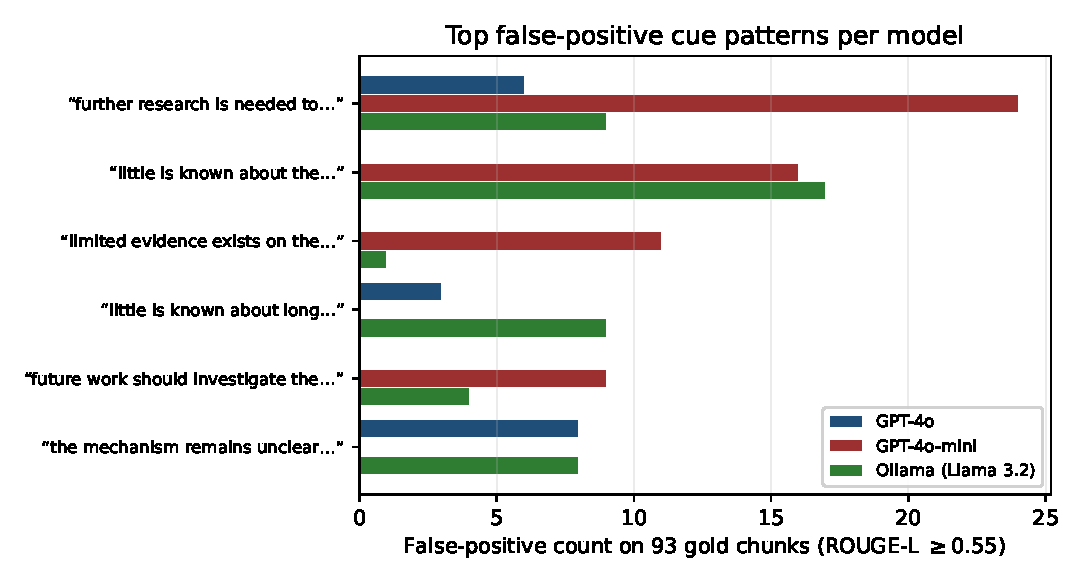
\includegraphics[width=0.92\linewidth]{figures/fp_patterns.pdf}
\caption{Top false-positive cue patterns per model (leading 5 words, lowercased, punctuation-stripped) on the $93$-chunk gold set at ROUGE-L $0.55$. The two smaller models over-generate \emph{``further research is needed to\ldots''} and \emph{``little is known about\ldots''} far more often than GPT-4o; that over-generation is the dominant driver of the precision gap in Table~\ref{tab:explicit}. Source: \texttt{Part2\_Output/fp\_patterns.csv}.}
\label{fig:fppat}
\end{figure}

\paragraph{Verbatim examples (from \texttt{Part2\_Output/error\_analysis.md}).}
\begin{quote}\small
\textbf{Representative false positive (chunk~50, GPT-4o-mini):} ``Further research is needed to replicate these findings.'' The post-filter regex accepts this sentence, but ROUGE-L cannot match it to any specific gold sentence in the chunk, so it counts as one FP for every chunk where the model emits it. This pattern alone accounts for \textbf{24} FPs in the GPT-4o-mini analysis.\\[2pt]
\textbf{Representative false negative (gold sentence in chunk~197):} ``Baillon et al., 2020.'' This is a citation fragment that PDF extraction merged into the body; it is not a knowledge-gap statement at all. Part-3 \texttt{clean-gold} removes seven such entries; we keep the uncleaned gold for the headline numbers in Table~\ref{tab:explicit} so the numbers stay comparable to GAPMAP's reporting.
\end{quote}
The FP/FN asymmetry (148 vs 18 for the two smaller models) is itself the story: they find nearly all the real gaps but pad output with cue-shaped non-gaps that the post-filter cannot reject (the regex was designed to admit cue phrases, not to verify a specific gold sentence is present).

\subsection{Paired ablations on the open-weight model}
Both precision/recall knobs documented in Section~\ref{sec:methods} (post-filter, hybrid merge) are measured here on the open-weight model at zero API cost. Table~\ref{tab:ollama-ablation} reports both. Panel~A (post-filter, paired on the same raw outputs) confirms that the post-filter is a precision floor; panel~B (hybrid merge, paired on the same filter-ON outputs) shows that the rule-based extractor adds nothing on top.

\begin{table}[h]
\centering
\caption{Paired ablations on Ollama Llama~3.2, same 93 gold chunks. \emph{Panel A} (post-filter): re-ran Ollama on the gold subset with prompt budget $3{,}500$ chars (vs.\ $8{,}000$ in Table~\ref{tab:explicit}, for local-Mac tractability) and evaluated the same raw outputs with and without the filter. \emph{Panel B} (hybrid merge): used the on-disk \texttt{predictions\_ollama.csv} (filter ON, full $8{,}000$-char budget) and unioned each chunk's predictions with \texttt{rule\_based\_extract} applied to chunk text. Sources: \texttt{ablation\_ollama\_postfilter.txt}, \texttt{ablation\_ollama\_hybrid.txt}.}
\label{tab:ollama-ablation}
\begin{tabular}{lrrrrrr}
\toprule
Config & TP & FP & FN & P & R & F1 \\
\midrule
\multicolumn{7}{l}{\textit{Panel A. Post-filter ablation (paired, prompt budget $3{,}500$ chars)}} \\
post-filter OFF (raw)              & 41  & 289 &  98 & 0.1242 & 0.2950 & 0.1748 \\
post-filter ON  (same raw)         & 37  &  97 & 100 & 0.2761 & 0.2701 & 0.2731 \\
$\Delta$ (ON $-$ OFF)              & $-4$ & $-192$ & $+2$ & $+0.1519$ & $-0.0249$ & $+0.0983$ \\
\midrule
\multicolumn{7}{l}{\textit{Panel B. Hybrid-merge ablation (paired, prompt budget $8{,}000$ chars, filter ON)}} \\
hybrid OFF (= Table~\ref{tab:explicit} Ollama row) & 151 & 148 & 20 & 0.5050 & 0.8830 & 0.6426 \\
hybrid ON  (filter ON $+$ \texttt{rule\_based})    & 151 & 148 & 20 & 0.5050 & 0.8830 & 0.6426 \\
$\Delta$ (ON $-$ OFF), $1{,}000$-bootstrap         & $0$ & $0$ & $0$ & $\pm 0.0000$ & $\pm 0.0000$ & $\pm 0.0000$ \\
\bottomrule
\end{tabular}
\end{table}

\paragraph{Panel A interpretation (post-filter as precision floor).} Reading the table top-to-bottom (filter OFF $\to$ ON, i.e., applying the filter): FP count drops from $289$ to $97$ ($3.0\times$ reduction), precision rises from $0.124$ to $0.276$, and F1 rises from $0.175$ to $0.273$. The cost is small: recall slips from $0.295$ to $0.270$ (a $0.025$ drop) because the filter rejects four true-positive sentences whose phrasing falls outside the cue regex. The post-filter therefore contributes $+0.152$ precision and $+0.098$ F1 at near-trivial recall cost. The prompt-budget reduction (3{,}500 vs.\ 8{,}000 chars) puts absolute numbers below Table~\ref{tab:explicit}'s on-disk Ollama row (F1 $=0.6426$); the paired \emph{delta} is what isolates the filter effect, and that delta is the scientifically valid claim.

\paragraph{Panel B interpretation (hybrid merge has zero effect).} Across $1{,}000$ bootstrap resamples of the 93 gold chunks, the rule-based extractor adds \emph{zero} new TPs, FPs, or FNs on top of filter-ON Ollama predictions. The reason is structural: the rule extractor uses the same cue regex as the post-filter, applied to chunk text rather than LLM output. Any cue-regex-matching sentence the rule extractor would surface is already in Ollama's filter-ON output (Ollama has near-perfect recall on cue-shaped sentences once the prompt asks for them). The remaining 20 FNs are gold sentences that do \emph{not} match the cue regex (citation fragments, low-saliency gaps not phrased as cues), and the rule extractor cannot find them either. The hybrid merge as currently implemented is therefore redundant on this corpus; raising recall on those 20 FNs requires either expanding the cue regex or moving them to the implicit (TABI) track.

\subsection{Implemented fixes and why they are justified}
\begin{itemize}
  \item \textbf{Gold cleaning (\texttt{clean-gold})}: removes citation-like gold sentences to reduce false negatives caused by non-gap gold noise.
  \item \textbf{Semantic-augmented scoring}: separates ``ROUGE-L paraphrase mismatch'' (which it can fix) from ``no gold sentence to match'' (which it cannot), giving a quantitative ceiling on how much of the precision gap is metric noise; we keep ROUGE-L as the rubric metric and use semantic-augmented only as a diagnostic.
  \item \textbf{TABI + entailment + threshold exports}: addresses implicit-gap \emph{over-generation} by producing a smaller set of claims with stronger automatic support checks, analogous in spirit to GAPMAP's emphasis on structured implicit reasoning and validation---though we do not claim equivalence to their biomedical implicit benchmark without a human implicit gold set.
  \item \textbf{Rule-based-only baseline (Table~\ref{tab:explicit}, top row)}: the no-LLM baseline calibrates how much of the chunk-level F1 number is achievable from the cue regex alone. Without this row a reader cannot tell whether the LLM is doing real work; with it, the LLM contribution is clearly attributable (a small unique-gold recall lift, paid for in precision) and the headline framing changes from ``LLMs do explicit gap extraction'' to ``LLMs are useful for paraphrase recall on explicit gaps and are required for the implicit (TABI) track.''
\end{itemize}

\subsection{Threats to validity}\label{sec:threats}
We consolidate the most reviewer-vulnerable caveats here so they can be evaluated together rather than scattered across the paper.

\paragraph{Metric (ROUGE-L per-prediction TP counting).} As implemented (and in alignment with GAPMAP's reporting), every prediction that matches \emph{any} gold sentence at ROUGE-L $\ge 0.55$ counts as a separate TP, even if multiple predictions hit the same gold sentence. Verbose models therefore inflate TPs while terse extractors do not. Our rule-based-only baseline (Table~\ref{tab:explicit}, top row) makes this concrete: it matches one fewer unique gold sentence than the LLMs ($110$ vs.\ $111$) but reports a higher F1, purely because the LLMs' duplicate-paraphrase TPs are counter-balanced by FPs. Quantifying paraphrase noise in the other direction, the semantic-augmented diagnostic (Table~\ref{tab:sem}) bounds the metric's \emph{undercount} of correct paraphrases at $\le +0.027$ F1.

\paragraph{Single-journal corpus and single-domain cue regex.} JBEE behavioral economics articles produce dense explicit-cue language; the $0.99$ precision of the rule-based baseline likely degrades on corpora where authors mark gaps less explicitly (e.g., theoretical economics, finance). The cue regex itself (Appendix~\ref{app:postfilter}) was not tuned to a held-out domain.

\paragraph{Single-annotator gold (explicit and implicit).} Gold gap sentences and the 20-row TABI spot-check were produced by one author using the cue regex as a seed (Section~\ref{sec:methods}). Inter-annotator agreement is unmeasured. The 70\% TABI real-gap rate in particular has no CI and should be read as an order-of-magnitude estimate.

\paragraph{Ablation budget asymmetry.} The Ollama post-filter ablation (Table~\ref{tab:ollama-ablation}, panel A) was run with a $3{,}500$-char prompt budget for local-Mac tractability versus $8{,}000$ chars for the on-disk Ollama row in Table~\ref{tab:explicit}; absolute F1 differs, but the paired \emph{delta} (the scientifically valid claim) is unaffected. The GPT post-filter ablation was not run because the cost of doubling our paid GPT-4o usage was unjustified given that the open-weight ablation already isolates the filter's effect.

\paragraph{TABI extraction model dependence.} The Part~3 TABI prompt is run with GPT-4o by default; we did not measure how MNLI pass rates or spot-check accuracy change if TABI is run with a smaller model. The validated/high-confidence row counts (842 / 784) should therefore be read as ``what GPT-4o $+$ MNLI yields on this corpus,'' not as model-agnostic numbers.

\section{Comparison to GAPMAP (what is comparable)}
\label{sec:vs-gapmap}
Table~\ref{tab:gapmap-vs-ours} situates our explicit numbers next to GAPMAP's reported results on policy/biodiversity assessments \citep{salem2025gapmap,ipbes2019global}. The corpora, gold construction, and our cue post-filter all differ; the correct scientific statement is \textbf{methodological alignment} (chunking + ROUGE-L $0.55$) plus qualitative agreement that frontier closed models are strong and open models remain useful. For implicit gaps, GAPMAP reports accuracy on curated biomedical implicit annotations; our MNLI pass rates and TABI spot-check are \textbf{internal validation statistics} (and a single-annotator order-of-magnitude estimate), not a reproduced benchmark accuracy.

\begin{table}[h]
\centering
\caption{Method-aligned but corpus-different comparison. ``Ours'' is on 93 JBEE chunks; GAPMAP's column is from Salem et al.\ Table~3 on policy/biodiversity text.}
\label{tab:gapmap-vs-ours}
\begin{tabular}{lcc}
\toprule
Model & Ours (JBEE, F1) & GAPMAP (policy, F1) \\
\midrule
GPT-4o      & $0.8822$ & $\approx 0.74$ \\
GPT-4o-mini & $0.6971$ & $\approx 0.81$ \\
Llama~3 family (open) & $0.6426$ & --- \\
\bottomrule
\end{tabular}
\end{table}

\section{Limitations and ethics}
\noindent The most reviewer-vulnerable methodological caveats (metric, single-journal, single-annotator, ablation budget, TABI model dependence) are consolidated in \S\ref{sec:threats}. Two further considerations are scope/ethics-oriented and live here.

\textbf{Hybrid merge.} As currently implemented, the rule-based merge re-uses the same cue regex as the post-filter and therefore adds zero on top of filter-ON LLM output (Table~\ref{tab:ollama-ablation} panel B). A non-trivial recall-boosting variant would need patterns the LLM does \emph{not} already produce.

\textbf{API cost and reproducibility.} Full-corpus TABI and the GPT explicit runs require paid API access; we mitigate failures with resume logic and pre-flight checks in \texttt{run\_part3.py}. The Ollama ablations, the rule-based baseline, the bootstrap CIs, and both figures (\path{run_baseline_and_figs.py}) require neither paid API access nor any GPU not present on a recent MacBook.

\textbf{Ethics.} The corpus is published peer-reviewed text used here for evaluation only; we do not redistribute the PDFs, and the TABI extraction outputs are claim candidates about \emph{authors' own stated limitations}, not new factual claims about third parties.

\section{Conclusion}
\label{sec:concl}
We deliver a reproducible explicit knowledge-gap baseline aligned with GAPMAP's ROUGE-L recipe, compare open- and closed-weight models on JBEE behavioral economics PDFs with bootstrap CIs, and extend the system with TABI-style implicit gap inference plus entailment-based calibration. On this corpus the most important calibration result is the no-LLM rule-based baseline (Table~\ref{tab:explicit}, top row): a cue-regex extractor with no model in the loop reaches F1 $=0.9091$ ($95\%$ CI $[0.849, 0.957]$) at $0.991$ precision, beating every LLM under chunk-level ROUGE-L. Among the LLMs, GPT-4o reaches F1 $=0.8822$ ($95\%$ CI $[0.838, 0.923]$) while GPT-4o-mini and Llama~3.2 cluster at $0.6971$ and $0.6426$ because both over-generate templated cue sentences that the post-filter cannot reject; the semantic-augmented diagnostic recovers at most $+0.027$ F1, confirming over-generation rather than paraphrase mismatch as the dominant failure mode. Two paired ablations on the open-weight model directly measure that (a) the post-filter contributes $+0.152$ precision / $+0.098$ F1 at a $-0.025$ recall cost, and (b) the hybrid rule merge adds zero on top of filter-ON LLM output across $1{,}000$ bootstrap resamples --- consistent with the rule-baseline finding (the LLM and the regex are recovering nearly the same set of unique gold sentences). The honest scientific takeaway is that on densely cue-marked behavioral-economics text, an LLM is not required for explicit gap extraction; the LLM's irreplaceable contribution is the implicit (TABI) track, where structured Claim/Grounds/Warrant inference and MNLI entailment validation produce candidates the regex cannot in principle reach.

\paragraph{Future work.} Four extensions are immediate and well-motivated by the findings above:
\begin{enumerate}
  \item \textbf{Domain shift away from cue-dense text.} Test whether the rule-based baseline still dominates on a less cue-marked corpus (e.g., theoretical-economics or finance journals) where ``further research is needed'' phrasing is rarer.
  \item \textbf{Metric reform.} Replace per-prediction TP counting with a unique-gold-coverage metric so verbose models cannot inflate F1 with paraphrase duplicates of the same gold sentence.
  \item \textbf{Implicit gold scale-up.} Scale the 20-row TABI spot-check (single annotator, $\sim 70\%$ real-gap rate) to a multi-annotator $100$--$200$-row implicit gold set so the TABI$+$MNLI track can be reported with a real P/R/F1 benchmark comparable to GAPMAP's biomedical implicit table.
  \item \textbf{Non-redundant hybrid merge.} Replace the current rule-merge (which re-uses the post-filter regex and adds zero on top, Table~\ref{tab:ollama-ablation} panel B) with cue patterns the LLM does \emph{not} already produce---e.g., implicit gap markers found by TABI but missed by the explicit cue regex.
\end{enumerate}

\section*{Software artifacts}
\noindent All code, notebooks, and data outputs are organized as follows so a grader can reproduce each table and figure from a single file.

\paragraph{Pipeline scripts (project root).}
\begin{itemize}
  \item \path{run_part2.py} --- explicit pipeline (extract, score, threshold sweep). \texttt{--error-analysis} writes per-model FP/FN files.
  \item \path{run_part3.py} --- Part~3 utilities (gold cleaning, semantic-augmented scoring, agreement export, TABI extraction/validation/high-confidence export).
  \item \path{annotate_gold_standard.py} --- rule-based seeding for gold annotation; uses the same cue regex as the post-filter.
  \item \path{run_ollama_ablation.py} --- paired post-filter ablation on Ollama (Table~\ref{tab:ollama-ablation} panel A; \path{Part2_Output/ablation_ollama_postfilter.txt}).
  \item \path{run_bootstrap_and_hybrid.py} --- 1{,}000-sample chunk-level bootstrap CIs (Table~\ref{tab:explicit}) and paired hybrid-merge ablation (Table~\ref{tab:ollama-ablation} panel B).
  \item \path{run_baseline_and_figs.py} --- rule-based-only baseline (Table~\ref{tab:explicit} top row), bootstrap-distribution figure (Figure~\ref{fig:bootf1}), and FP-pattern figure (Figure~\ref{fig:fppat}).
  \item \path{Part3_Output/tabi_spotcheck_template.py} --- stratified TABI spot-check sampler (20-row implicit gap audit).
\end{itemize}

\paragraph{Notebooks.} \path{Part2_Explicit_Gap_Extraction.ipynb}, \path{Part3_GAPMAP_Extensions.ipynb}.

\paragraph{Bibliography.} \path{Final_Paper/references.bib} (in-line citations $+$ \texttt{nocite} corpus block).

\paragraph{Generated data outputs.}
\begin{itemize}
  \item \path{Part2_Output/} summary text files: \path{comparison_results.txt}, \path{threshold_tuning.txt}, \path{bootstrap_ci.txt}, \path{baseline_rule_only.txt}, \path{ablation_ollama_postfilter.txt}, \path{ablation_ollama_hybrid.txt}.
  \item \path{Part2_Output/} CSVs: \path{bootstrap_samples.csv}, \path{fp_patterns.csv}, and per-method prediction files \path{predictions_<model>.csv} including \path{predictions_rule_only.csv} for the no-LLM baseline.
  \item \path{Part2_Output/} per-model error analysis: primary \path{error_analysis.md} plus siblings for each LLM (\texttt{error\_analysis\_gpt\_4o.md}, etc.).
  \item \path{Part3_Output/} (a): \path{semantic_compare.txt}, \path{high_confidence_chunks.csv}, \path{tabi_spotcheck_20.csv}.
  \item \path{Part3_Output/} (b) TABI CSV family --- four files prefixed \texttt{tabi\_}: \texttt{outputs}, \texttt{outputs\_validated}, \texttt{high\_confidence\_mnli06}, \texttt{high\_confidence\_mnli07}.
  \item \path{Final_Paper/figures/}: \path{bootstrap_f1.pdf} (Figure~\ref{fig:bootf1}), \path{fp_patterns.pdf} (Figure~\ref{fig:fppat}).
\end{itemize}

\appendix
\section{Reproducibility commands}
\noindent Commands assume the project root contains the PDF corpus, Python~3.11+, \path{OPENAI_API_KEY} for API-backed steps, and Ollama for local Llama runs. Exact paths depend on your machine; the course bundle uses the repository layout documented in \path{Final_Paper/README.md}. The committed \path{Part2_Output/comparison_results.txt}, \path{Part2_Output/threshold_tuning.txt}, \path{Part2_Output/error_analysis.md}, and \path{Part3_Output/semantic_compare.txt} were all regenerated from the current prediction CSVs, so a fresh \texttt{run\_part2.py --compare} reproduces Table~\ref{tab:explicit} verbatim.

\begin{verbatim}
# Part 2: extract + compare (after predictions exist)
python run_part2.py --compare
python run_part2.py --threshold-tuning
python run_part2.py --error-analysis    # per-model FP/FN files

# Part 3: gold hygiene, semantic scores, agreement, TABI
python run_part3.py clean-gold
python run_part3.py semantic-compare
python run_part3.py export-agreement
python run_part3.py tabi-extract
python run_part3.py tabi-validate
python run_part3.py tabi-high-confidence --mnli-threshold 0.6
python run_part3.py tabi-high-confidence --mnli-threshold 0.7

# Bootstrap CIs + paired hybrid ablation (no API, no Ollama; ~1 min):
python run_bootstrap_and_hybrid.py
# Outputs: Part2_Output/bootstrap_ci.txt, ablation_ollama_hybrid.txt

# Rule-based baseline + Figures 2, 3 (no API, no Ollama; ~1 min):
python run_baseline_and_figs.py
# Outputs: Part2_Output/baseline_rule_only.txt, bootstrap_samples.csv,
#          fp_patterns.csv, predictions_rule_only.csv,
#          Final_Paper/figures/bootstrap_f1.pdf, fp_patterns.pdf

# Post-filter ablation (local Ollama; Apple Silicon: ~2 min):
ollama serve &
OLLAMA_ABLATION_N=93 python run_ollama_ablation.py
# Output:  Part2_Output/ablation_ollama_postfilter.txt
\end{verbatim}

\section{Post-filter regular expressions}
\label{app:postfilter}
\noindent The cue-phrase post-filter applied during explicit extraction (Section~\ref{sec:methods}, ``Post-filter'') is implemented in \texttt{run\_part2.py} as \texttt{filter\_predictions}, which keeps a predicted sentence if and only if any of the patterns below matches case-insensitively. The same set is used by \texttt{rule\_based\_extract} for the (optional) hybrid merge and by \texttt{annotate\_gold\_standard.py} for rule-based seeding. We list it here so a grader can verify exactly which sentences the filter admits and rejects.

\begin{verbatim}
GAP_PATTERNS = [
    r"remains unknown", r"remains unclear", r"it is unclear",
    r"it remains unclear",
    r"further research (is )?needed", r"further research (is )?required",
    r"more research (is )?needed", r"limited evidence",
    r"no study has", r"no studies have",
    r"notable gaps remain", r"future work should", r"future research should",
    r"we lack (data|evidence|information)", r"little is known",
    r"poorly understood",
    r"remains (to be )?explored",
    r"merits further (study|research)",
    r"warrants further (study|research)",
    r"open (question|questions)", r"unresolved",
    r"under-researched", r"understudied",
    r"scant evidence", r"scarce (evidence|data)",
    r"inconclusive", r"mixed evidence",
    r"may lead to unintended",
]
\end{verbatim}

\noindent The set is intentionally inclusive: it admits cue \emph{shapes} (verbatim limitations / future-work language) without verifying that a specific gold sentence exists in the chunk. This is exactly why the post-filter acts as a precision floor (Section~\ref{sec:fail}, Table~\ref{tab:ollama-ablation} panel A) rather than a precision ceiling, and why the rule-merge built from the same regex adds nothing on top (panel B).

\section{Corpus list (107 articles)}\label{app:corpus}
\noindent The complete inventory of the 107 \emph{Journal of Behavioral and Experimental Economics} articles used to build the 1{,}367-chunk corpus is provided in the supplementary file \path{Part3_Output/Appendix_A_Expanded_Corpus_URLs.md}. That file lists every article as a row keyed by its BibTeX identifier (\texttt{jbee\_pdf\_001}--\texttt{jbee\_pdf\_113}, with the six editorial-board entries excluded), together with publication year, title slug, and local corpus path; it also records the journal hubs from which the corpus was sourced and a reproducibility note for re-assembling it. To keep the main bibliography readable, individual \texttt{BibTeX} entries for each corpus PDF (\texttt{jbee\_pdf\_001}--\texttt{jbee\_pdf\_113}) are kept in \path{Final_Paper/references.bib} but are not listed in the \emph{References} section: they are not inline-cited and would otherwise crowd out the methodological citations.

\bibliographystyle{plainnat}
\bibliography{references}

\end{document}
